\section{Cobordism 1}
Suppose we have 
\begin{itemize}
\item a punctured Riemann sphere $M$

\item co-oriented link $\Lambda_0 = (\Phi_0,\xi_0)$ about $0$

\item co-oriented link $\Lambda_\infty = (\Phi_\infty,\xi_\infty)$ about $\infty$ 

\item a co-oriented lines $\Lambda_{squig} = (\Phi_{squig}, \xi_{squig})$ that refines the stratification induced by $\Lambda_0 \coprod \Lambda_\infty$ to a regular cell complex 
\end{itemize}
and suppose we have a nested disk $D' \subset D \subset M$ and a smooth chart
\[
	f: \{(x,z)\in \R^2 ~|~ x^2+z^2 < 4 \} \rightarrow D
\]
such that 
\begin{itemize}
\item $\{(x,z)\in \R^2 ~|~ x^2+z^2 < 1\}$ is mapped to $D'$ 

\item I will abuse the notation so that $D'$ denotes $\{(x,z)\in \R^2 ~|~ x^2+z^2 < 1\}$ and $D$ denotes $\{(x,z)\in \R^2 ~|~ x^2+z^2 < 4 \}$

\item $\{(x,z)\in D' ~|~ z = \frac{1}{2} \}$, co-oriented downward, is mapped to $\Lambda_0 |_{D'}$

\item $\{(x,z)\in D' ~|~ z = -\frac{1}{2} \}$, co-oriented upward, is mapped to $\Lambda_\infty |_{D'}$

\item $\{(x,z)\in D' ~|~ x = 0 \}$, co-oriented leftward, is mapped to $\Lambda_{squig} |_{D'}$
\end{itemize}
\begin{definition}
Let $m,n \in \N$ and $0\leq k \leq n$, then we define $iota_k$ to be
	\begin{align*}
		\iota_k : & ~ \C^{m} \rightarrow \C^{m+n} \\
		& ~ e_i \mapsto e_{i+k}
	\end{align*}
	where $e_i$ is the $i^{th}$ standard basis vector of $\C^m$ and $\C^{m+n}$		
\end{definition}
Suppose we have a sheaf $\mathfrak{F}$ singular supported on $\Lambda_0 \coprod \Lambda_\infty \coprod \Lambda_{squig}$, $f^*\mathfrak{F}$ is described as the following legible diagram.

\begin{definition}
Let $sgn:~\R \rightarrow \{-,0,+\}$ where
\[
sgn(x) = \begin{cases}
    - & \text{if } x < 0 \\
    0 & \text{if } x = 0 \\
    + & \text{if } x > 0
\end{cases}
\]
\end{definition}
\begin{definition}
\[
s_0(sgn_1,sgn_2,sgn_3):=~ \{(x,z) \in D' ~|~ sgn(z-\frac{1}{2})=sgn_1,~ sgn(-\frac{1}{2}-z)=sgn_2,~ sgn(x)=sgn_3 \}
\]
\end{definition}

Note that $\Lambda_0 \coprod \Lambda_\infty \coprod \Lambda_{squig}$ divides $D'$ into $6$ regions which are
\[
	s_0(+,-,-),s_0(+,-,+),s_0(-,+,-),s_0(-,+,+),s_0(-,-,-),s_0(-,-,+)
\]

The legible diagram for $f^*\mathfrak{F}$ is given as follows\\
\textbf{Stalks:}
\begin{itemize}
\item $F_0(s_0(-,-,sgn_3))$ := $\mathbb{C}^{m}$
\item $F_0(s_0(+,-,sgn_3))$ := $\mathbb{C}^{m+1}$
\item $F_0(s_0(-,+,sgn_3))$ := $\mathbb{C}^{m+1}$
\end{itemize}
where $sgn_3 \in \{-, + \}$.\\
\textbf{Generization maps:}
\begin{itemize}
\item $F_0(s_0(0,sgn_2,sgn_3)):~ F_0(s_0(-,sgn_2,sgn_3))\rightarrow F_0(s_0(+,sgn_2,sgn_3))$ := $\iota_1$ 

\item $F_0(s_0(sgn_1,0,sgn_3)):~ F_0(s_0(sgn_1,-,sgn_3))\rightarrow F_0(s_0(sgn_1,+,sgn_3))$ := $\iota_0$ 

\item $F_0(s_0(-,-,0)):~ F_0(s_0(-,-,-))\rightarrow F_0(s_0(-,-,+))$ := $T(2,2,m+1,m+1)$ 

\item $F_0(s_0(+,-,0)):~ F_0(s_0(+,-,-))\rightarrow F_0(s_0(+,-,+))$ := $T(2,2,m+2,m+2)$ 

\item $F_0(s_0(-,+,0)):~ F_0(s_0(-,+,-))\rightarrow F_0(s_0(-,+,+))$ := $T(1,1,m+1,m+1)$ 
\end{itemize}
Here, $T$ is a matrix that gives rise to a linear transformation from $\C^{m+2}$ to $\C^{m+2}$ where
\begin{itemize}
\item $T(span\{ e_2, \cdots, e_{m+1} \}) \subset span\{ e_2, \cdots, e_{m+1} \}$

\item $T(span\{ e_1, \cdots, e_{m+1} \}) \subset span\{ e_1, \cdots, e_{m+1} \}$

\item $T(span\{ e_2, \cdots, e_{m+2} \}) \subset span\{ e_2, \cdots, e_{m+2} \}$
\end{itemize}
and $T(r_{start},r_{end},c_{start},c_{end})$ is the submatrix of $T$ that contains rows from $r_{start}$ to $r_{end}$ and columns from $c_{start}$ to $c_{end}$.\\

Now I will define a cobordism of $f^*\mathfrak{F}$, say $Cobordism_1$ that satisfies the following conditions
\begin{itemize}
\item $Cobordism_1$ is supported on $overline{D}$

\item $Cobordism_1$ inside of $D-D'$ is perturbed so that $\Lambda$'s remain smooth link throughout the isotopy but won't exactly describe what it is

\item I will only describe $Cobordism_1$ inside $D'$
\end{itemize}
Now let's define $Cobordism_1$ as a legible diagram on $D'\times [0,1]_t$ whose regions are the regions separated by the following hyperplanes corresponding to the world sheets of $\Lambda_0$, $\Lambda_\infty$, and $\Lambda_{squig}$
\begin{itemize}
\item world sheet of $\Lambda_0$: 
$\{(x,z,t) \in D' \times [0,1] ~|~ z=\frac{5}{3}tx^2 + \frac{5}{4}(1-t)-\frac{3}{4}\}$, where hairs are pointing downward. Note that when $t=t_0$, the above set is the parabola passing through $(-\frac{\sqrt{3}}{2}, \frac{1}{2})$, $(\frac{\sqrt{3}}{2}, \frac{1}{2})$, and $(0,-\frac{5}{4}t_0 + \frac{1}{2})$.

\item world sheet of $\Lambda_\infty$: 
$\{(x,z,t) \in D' \times [0,1] ~|~ z=-\frac{1}{2} \}$, where hairs are pointing upward.

\item world sheet of $\Lambda_{squig}$:
$\{(x,z,t) \in D' \times [0,1] ~|~ x=0 \}$, where hairs are pointing leftward.
\end{itemize}
\begin{definition}
\begin{align*}
s(sgn_1,sgn_2,sgn_3) :=~ &\{(x,z,t) \in D' \times [0,1] ~|~ sgn(z-\frac{5}{3}tx^2-\frac{5}{4}(1-t)+\frac{3}{4}) = sgn_1, \\
& sgn(-\frac{1}{2}-z)=sgn_2,sgn(x)=sgn_3
	\}
\end{align*}
\end{definition}
The above three world sheets separate $D'\times [0,1]$ into $8$ regions
\[
	\{s(sgn_1,sgn_2,sgn_3) ~|~ sgn_1,sgn_2,sgn_3 \in \{-,+\}\}
\]
and we get the following stratification
\[
	\mathcal{S} = \{ s(sgn_1,sgn_2,sgn_3) ~|~ sgn_1,sgn_2, sgn_3 \in \{-,0,+\} \}
\]
Now let's define a legible diagram $F$ as follows
\textbf{Stalks:}
\begin{itemize}
\item $F_0(s_0(-,-,sgn_3))$ := $\mathbb{C}^{m}$
\item $F_0(s_0(+,-,sgn_3))$ := $\mathbb{C}^{m+1}$
\item $F_0(s_0(-,+,sgn_3))$ := $\mathbb{C}^{m+1}$
\item $F_0(s_0(+,+,sgn_3))$ := $\mathbb{C}^{m+2}$
\end{itemize}
where $sgn_3 \in \{-, + \}$.\\
\textbf{Generization maps:}
\begin{itemize}
\item $F_0(s_0(0,sgn_2,sgn_3)):~ F_0(s_0(-,sgn_2,sgn_3))\rightarrow F_0(s_0(+,sgn_2,sgn_3))$ := $\iota_1$ 

\item $F_0(s_0(sgn_1,0,sgn_3)):~ F_0(s_0(sgn_1,-,sgn_3))\rightarrow F_0(s_0(sgn_1,+,sgn_3))$ := $\iota_0$ 

\item $F_0(s_0(-,-,0)):~ F_0(s_0(-,-,-))\rightarrow F_0(s_0(-,-,+))$ := $T(2,2,m+1,m+1)$ 

\item $F_0(s_0(+,-,0)):~ F_0(s_0(+,-,-))\rightarrow F_0(s_0(+,-,+))$ := $T(2,2,m+2,m+2)$ 

\item $F_0(s_0(-,+,0)):~ F_0(s_0(-,+,-))\rightarrow F_0(s_0(-,+,+))$ := $T(1,1,m+1,m+1)$ 

\item $F_0(s_0(+,+,0)):~ F_0(s_0(+,+,-))\rightarrow F_0(s_0(+,+,+))$ := $T$ 
\end{itemize}
Here, $T$ is a matrix that gives rise to a linear transformation from $\C^{m+2}$ to $\C^{m+2}$ where
\begin{itemize}
\item $T(span\{ e_2, \cdots, e_{m+1} \}) \subset span\{ e_2, \cdots, e_{m+1} \}$

\item $T(span\{ e_1, \cdots, e_{m+1} \}) \subset span\{ e_1, \cdots, e_{m+1} \}$

\item $T(span\{ e_2, \cdots, e_{m+2} \}) \subset span\{ e_2, \cdots, e_{m+2} \}$
\end{itemize}
and $T(r_{start},r_{end},c_{start},c_{end})$ is the submatrix of $T$ that contains rows from $r_{start}$ to $r_{end}$ and columns from $c_{start}$ to $c_{end}$.
\begin{definition}
Let $\mathcal{S}$ be a stratication of $D'\times[0,1]$ and let $s$ be a stratum in $\mathcal{S}$ of sub-penultimate dimension. Suppose we have a diagram $F$ assigning regions to vector spaces and penultimate dimensional strata to linear maps between bordering regions where the map goes against the co-orientation, then we defin the subdiagram associated to $s$ to be the diagram restricted to the regions incident with $s$ and maps between those regions.
\end{definition}

\begin{proposition}
The above diagram is a well-defined legible diagram.
\end{proposition}
\begin{proof}
It is enough to show that the total complexes of the subdiagrams the above defined diagram associated to sub-penultimate dimensional strata.\\
\textbf{(\RN{1}) $1$ dimensional strata:}
\begin{itemize}
\item subdiagram associated to $s(0,0,sgn_3)$ where $sgn_3 \in \{-,+\}$:\\
\begin{tikzcd}[row sep=2cm, column sep=2.5cm]
s(-,+,\text{sgn}_3) \arrow[r, "{s(0,+,\text{sgn}_3)}"] & s(+,+,\text{sgn}_3) \\
s(-,-,\text{sgn}_3) \arrow[r, "{s(0,-,\text{sgn}_3)}"]\arrow[u,"{s(-,0,\text{sgn}_3)}"] & s(+,-,\text{sgn}_3) \arrow[u,"{s(+,0,\text{sgn}_3)}"]
\end{tikzcd}
=
\begin{tikzcd}
\C^{m+1} \arrow[r, "{\iota_1}"] & \C^{m+2} \\
\C^{m} \arrow[r, "{\iota_1}"]\arrow[u,"{\iota_0}"] & \C^{m+1} \arrow[u,"{\iota_0}"]
\end{tikzcd}\\
whose total complex is
\[
\begin{tikzcd}
0 \arrow[r] & \C^{m+1} \arrow[r, "{\iota_0 \oplus \iota_1}"] & \C^{m+1} \oplus \C^{m+1} \arrow[r, "{-\iota_1 \oplus \iota_0}"] & \C^{m+2} \arrow[r] & 0
\end{tikzcd}
\]
where 
\begin{align*}
ker(-\iota_1 \oplus \iota_0) = & \{(u,v) \in \C^{m+1} \oplus \C^{m+1} ~|~ \iota_1(u) = \iota_0(v) \}\\
= & \{(u,v) \in \C^{m+1} \oplus \C^{m+1} ~|~ u_{m+1} = 0, v_1 = 0, u_i=v_{i+1}\text{ for }i=1,\cdots,m+1 \} \\
= & Im(\iota_0 \oplus \iota_1)
\end{align*}
Therefore, the total complex is acyclic.

\item subdiagram associated to $s(0,+,0)$:\\
\begin{tikzcd}[row sep=2cm, column sep=2.5cm]
s(+,+,-) \arrow[r, "{s(+,+,0)}"] & s(+,+,+) \\
s(-,+,-) \arrow[r, "{s(-,+,0)}"]\arrow[u,"{s(0,+,-)}"] & s(-,+,+) \arrow[u,"{s(0,+,+)}"]
\end{tikzcd}
=
\begin{tikzcd}[column sep=2.5cm]
\C^{m+2} \arrow[r, "{T}"] & \C^{m+2} \\
\C^{m+1} \arrow[r, "{T(2,2,m+2,m+2)}"]\arrow[u,"{\iota_1}"] & \C^{m+1} \arrow[u,"{\iota_1}"]
\end{tikzcd}\\

\item subdiagram associated to $s(0,-,0)$:\\
\begin{tikzcd}[row sep=2cm, column sep=2.5cm]
s(+,-,-) \arrow[r, "{s(+,-,0)}"] & s(+,-,+) \\
s(-,-,-) \arrow[r, "{s(-,-,0)}"]\arrow[u,"{s(0,-,-)}"] & s(-,-,+) \arrow[u,"{s(0,-,+)}"]
\end{tikzcd}
=
\begin{tikzcd}[column sep=2.5cm]
\C^{m+1} \arrow[r, "{T(1,1,m+1,m+1)}"] & \C^{m+1} \\
\C^{m} \arrow[r, "{T(2,2,m+1,m+1)}"]\arrow[u,"{\iota_1}"] & \C^{m} \arrow[u,"{\iota_1}"]
\end{tikzcd}\\

\item subdiagram associated to $s(+,0,0)$:\\
\begin{tikzcd}[row sep=2cm, column sep=2.5cm]
s(+,+,-) \arrow[r, "{s(+,+,0)}"] & s(+,+,+) \\
s(+,-,-) \arrow[r, "{s(+,-,0)}"]\arrow[u,"{s(+,0,-)}"] & s(+,-,+) \arrow[u,"{s(+,0,+)}"]
\end{tikzcd}
=
\begin{tikzcd}[column sep=2.5cm]
\C^{m+2} \arrow[r, "{T}"] & \C^{m+2} \\
\C^{m+1} \arrow[r, "{T(1,1,m+1,m+1)}"]\arrow[u,"{\iota_0}"] & \C^{m+1} \arrow[u,"{\iota_0}"]
\end{tikzcd}\\

\item subdiagram associated to $s(-,0,0)$:\\
\begin{tikzcd}[row sep=2cm, column sep=2.5cm]
s(-,+,-) \arrow[r, "{s(-,+,0)}"] & s(-,+,+) \\
s(-,-,-) \arrow[r, "{s(-,-,0)}"]\arrow[u,"{s(-,0,-)}"] & s(-,-,+) \arrow[u,"{s(-,0,+)}"]
\end{tikzcd}
=
\begin{tikzcd}[column sep=2.5cm]
\C^{m+1} \arrow[r, "{T(2,2,m+2,m+2)}"] & \C^{m+1} \\
\C^{m} \arrow[r, "{T(2,2,m+1,m+1)}"]\arrow[u,"{\iota_0}"] & \C^{m} \arrow[u,"{\iota_0}"]
\end{tikzcd}\\
\end{itemize}

\textbf{(\RN{2}) $0$ dimensional stratum:}
\begin{itemize}
\item diagram associated to $s(0,0,0)$:\\
\item \begin{tikzcd}[row sep=1.5cm, column sep=2cm]
& s(-,+,+)\arrow[dd,"{s(-,+,0)}"'] \arrow[rr,"{s(0,+,+)}"] & & s(+,+,+) \arrow[dd,"{s(+,+,0)}"']\\
s(-,-,+) \arrow[dd,"{s(-,-,0)}"']\arrow[rr,"{s(0,-,+)}"] \arrow[ur,"{s(-,0,+)}"] & & s(+,-,+) \arrow[dd,"{s(+,-,0)}"']\arrow[ur,"{s(+,0,+)}"']& \\
& s(-,+,-) \arrow[rr,"{s(0,+,-)}"'] & & s(+,+,-)  \\
s(-,-,-) \arrow[rr,"{s(0,-,-)}"'] \arrow[ur,"{s(-,0,-)}"] & & s(+,-,-) \arrow[ur,"{s(+,0,-)}"] &
\end{tikzcd}\\
=
\begin{tikzcd}[row sep=2cm, column sep=2.5cm]
& \C^{m+1} \arrow[rr,"{\iota_1}"] & & \C^{m+2} \\
\C^{m} \arrow[rr,"{\iota_1}"] \arrow[ur,"{\iota_0}"] & & \C^{m} \arrow[ur,"{\iota_0}"']& \\
& \C^{m+1} \arrow[rr,"{\iota_1}"']\arrow[uu,"{T(2,2,m+2,m+2)}"'] & & \C^{m+2} \arrow[uu,"{T}"'] \\
\C^{m} \arrow[rr,"{\iota_1}"'] \arrow[ur,"{\iota_0}"] \arrow[uu,"{T(2,2,m+1,m+1)}"']& & \C^{m+1} \arrow[ur,"{\iota_0}"] \arrow[uu,"{T(1,1,m+1,m+1)}"']&
\end{tikzcd}
\end{itemize}
\end{proof}
\begin{figure}[H] 
    \centering
    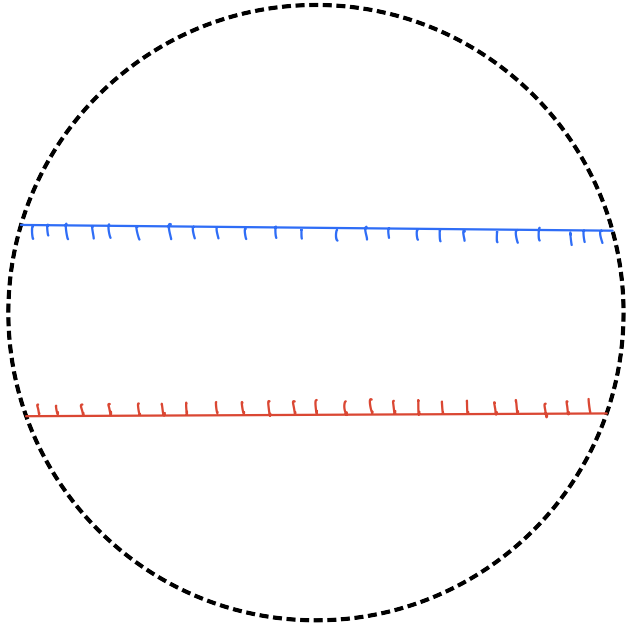
\includegraphics[scale = 0.95]{diagrams/lemma1/1.png} 
    \caption{Your caption here}
    \label{fig:your-label}
\end{figure}


\begin{figure}[H] 
    \centering
    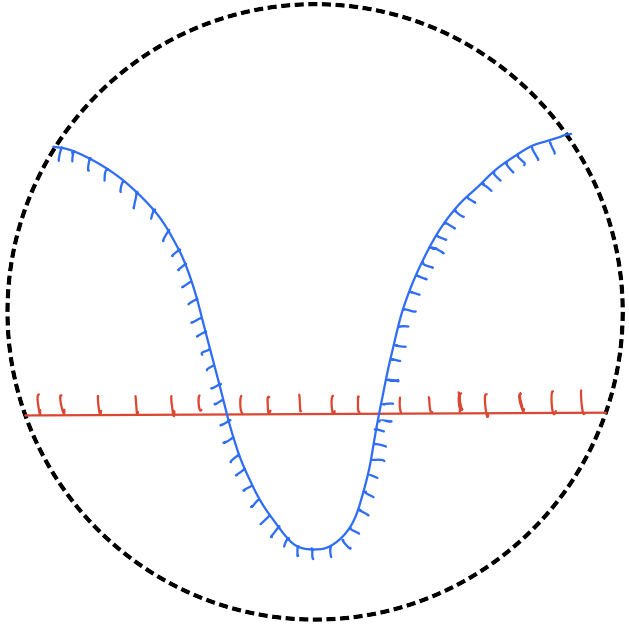
\includegraphics[scale = 0.95]{diagrams/lemma1/2.png} 
    \caption{Your caption here}
    \label{fig:your-label}
\end{figure}


\begin{figure}[H] 
    \centering
    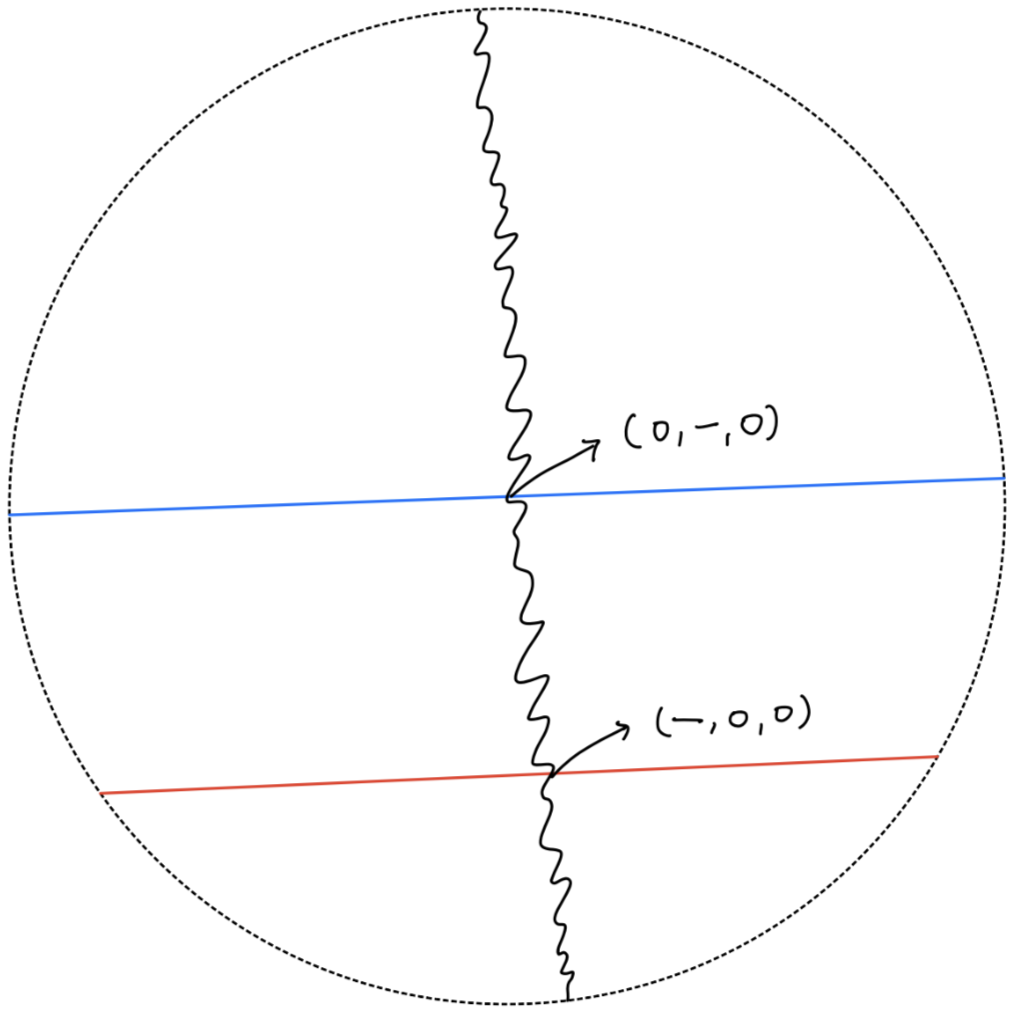
\includegraphics[scale = 0.95]{diagrams/lemma1/3.png} 
    \caption{Your caption here}
    \label{fig:your-label}
\end{figure}

\begin{figure}[H] 
    \centering
    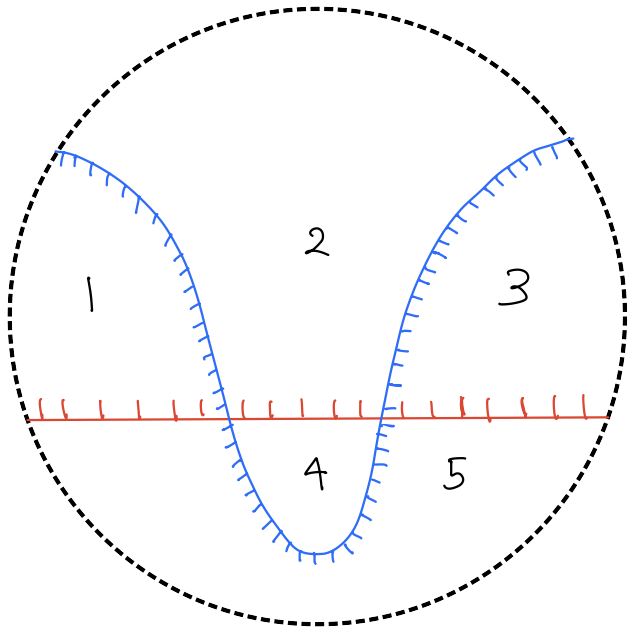
\includegraphics[scale = 0.95]{diagrams/lemma1/4.png} 
    \caption{Your caption here}
    \label{fig:your-label}
\end{figure}